%%% Local Variables:
%%% mode: latex
%%% TeX-master: "../doc"
%%% coding: utf-8
%%% End:
% !TEX TS-program = pdflatexmk
% !TEX encoding = UTF-8 Unicode
% !TEX root = ../doc.tex
\section{Aufgabenstellung}
\label{sec:aufgabenstellung}
\begin{figure}[H]
  \centering
  
\includegraphics[page=1,scale=0.55]{../ressources/Aufgabenstellung.pdf}
\end{figure}
\begin{figure}[H]
  \centering

\includegraphics[page=2,scale=0.55]{../ressources/Aufgabenstellung.pdf}
\end{figure}


\section{Packages}
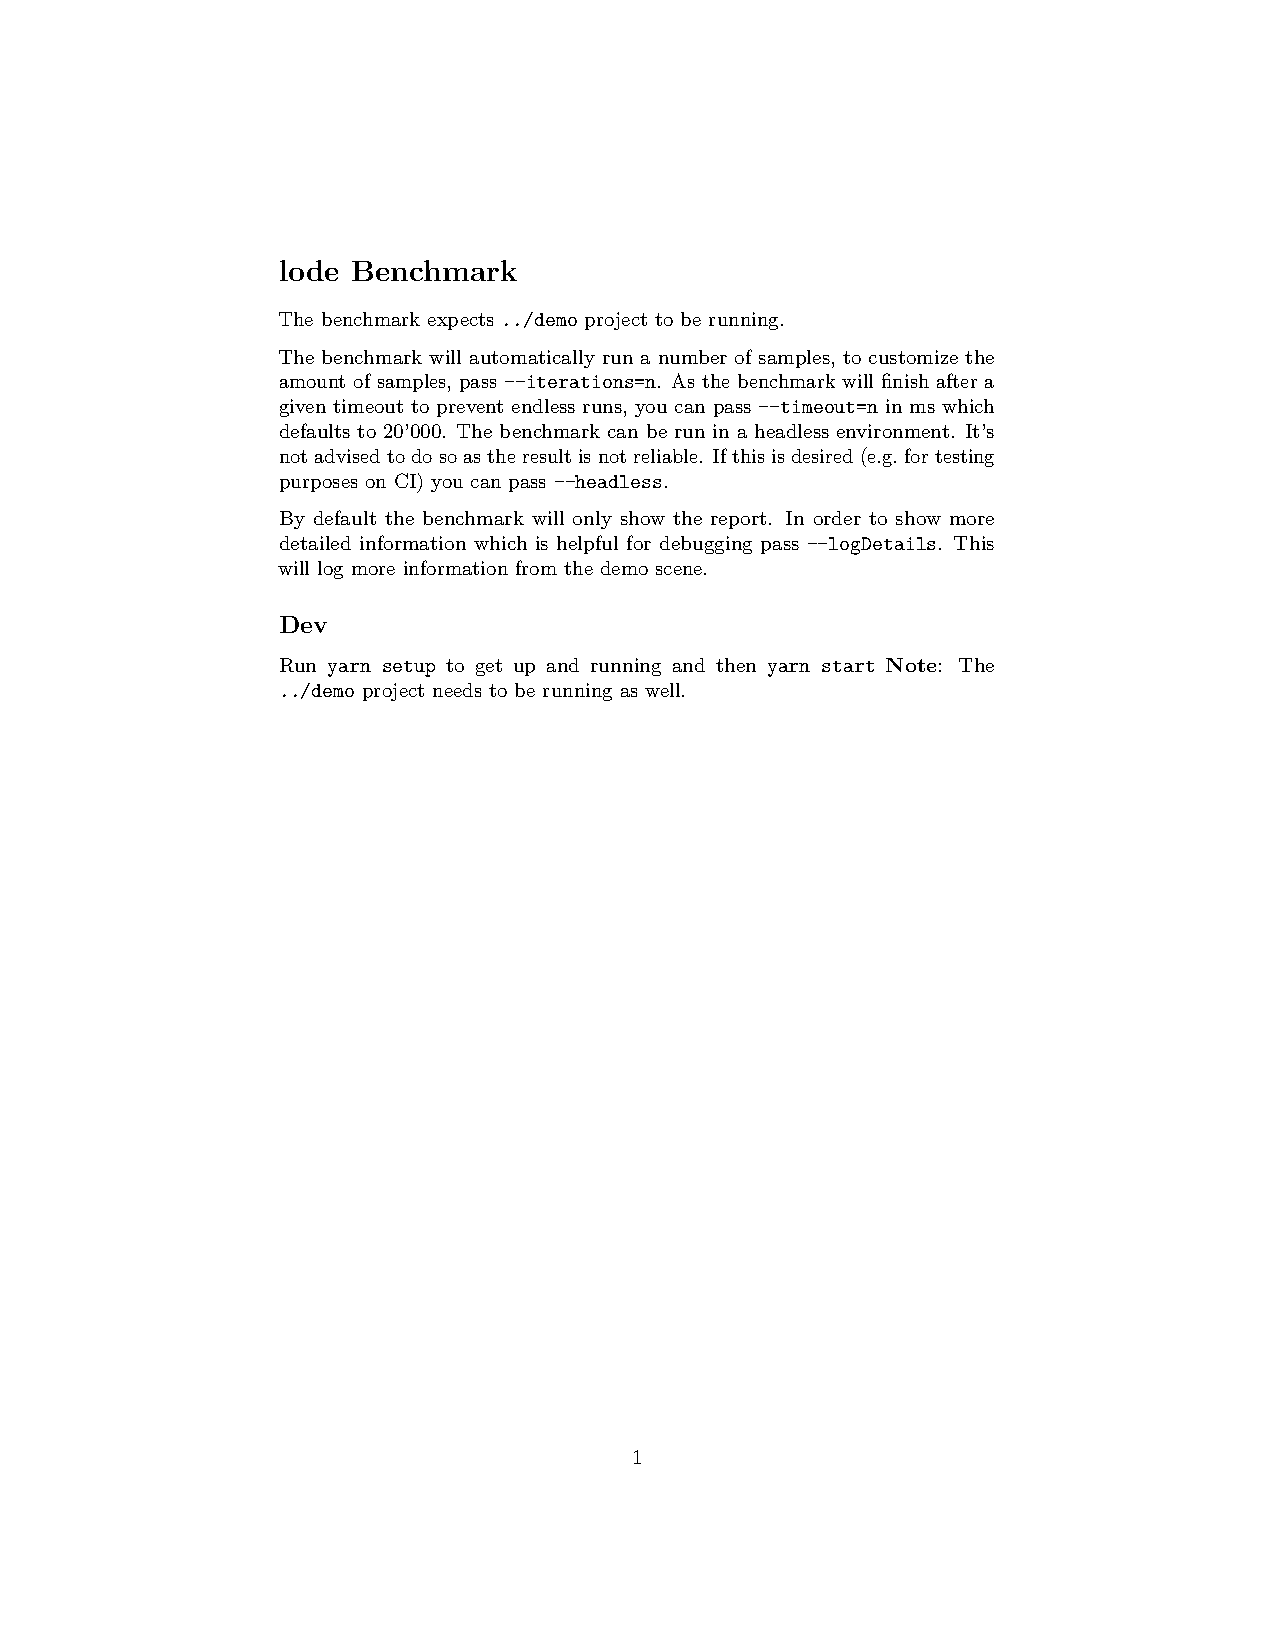
\includepdf[pagecommand={},scale=0.92,pages=-]{../ressources/packages/benchmark.pdf}
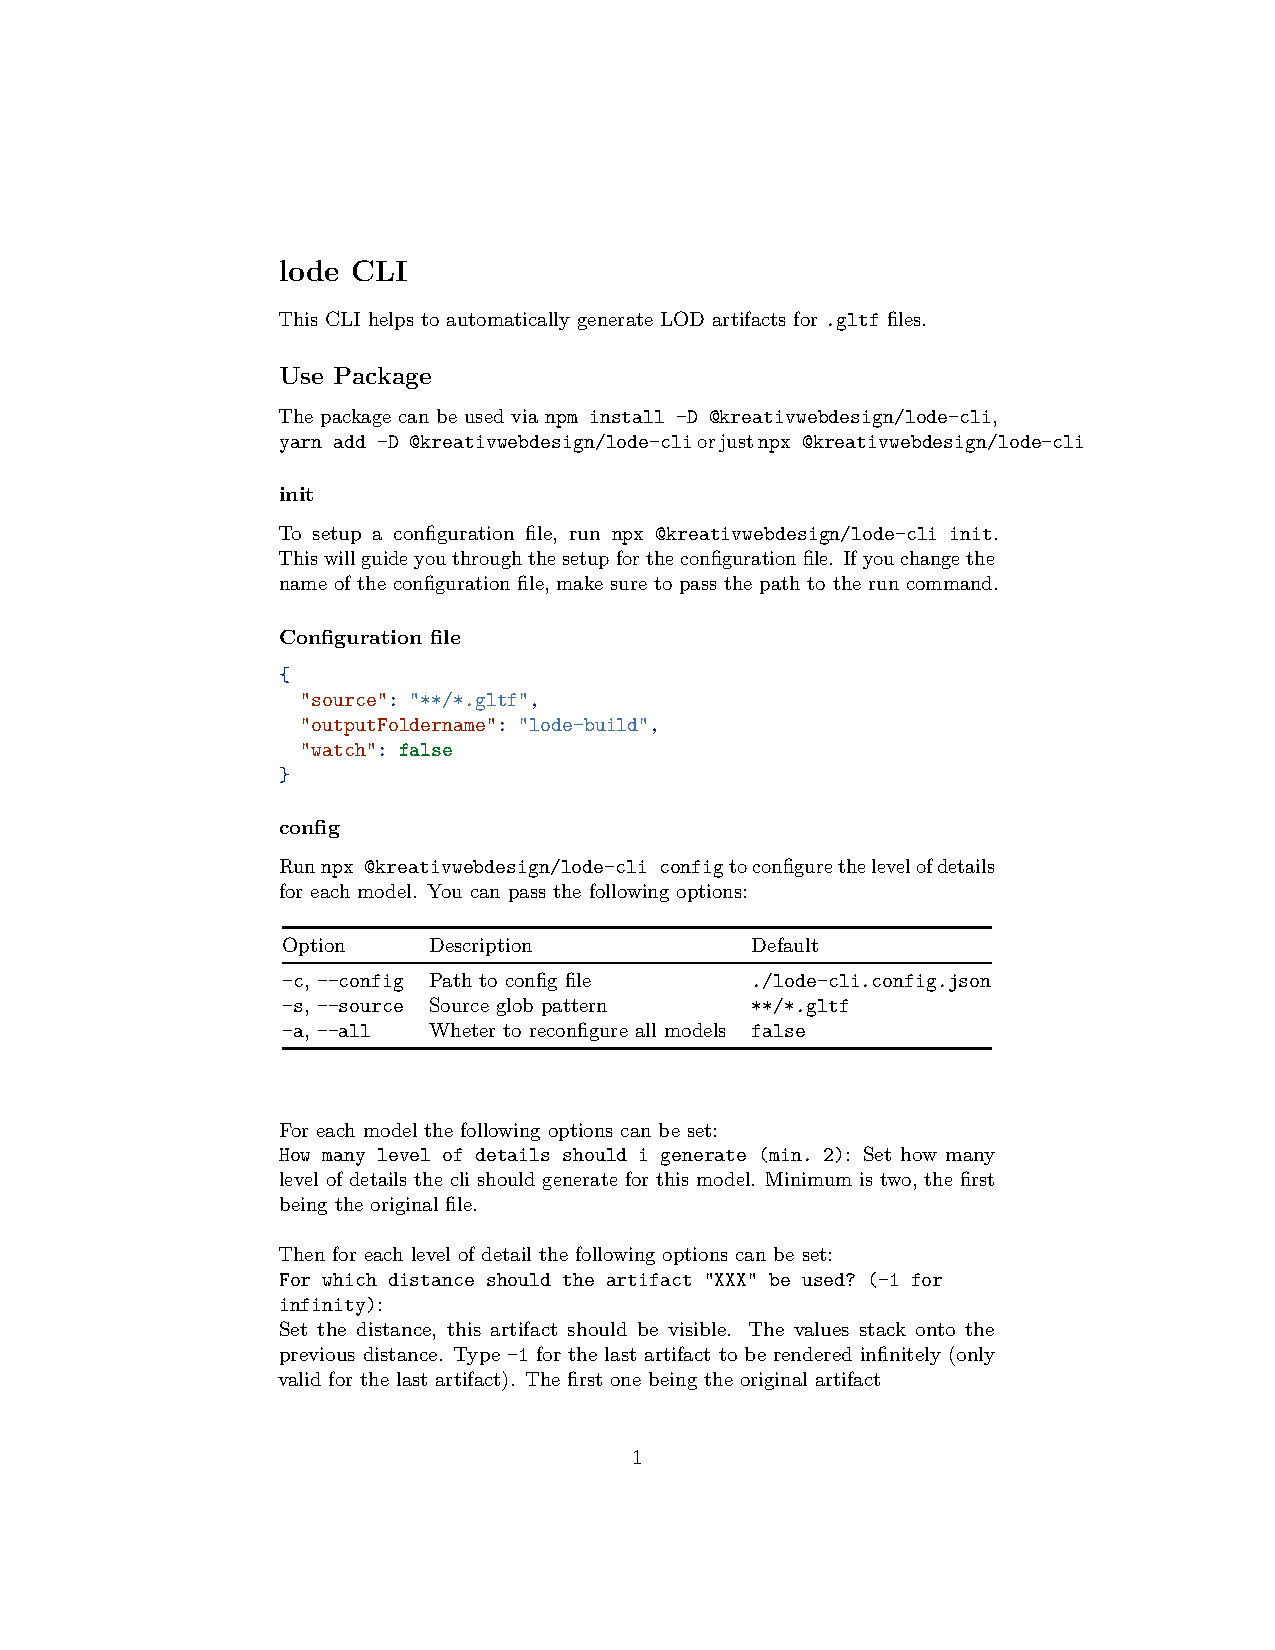
\includepdf[pagecommand={},scale=0.92,pages=-]{../ressources/packages/cli.pdf}
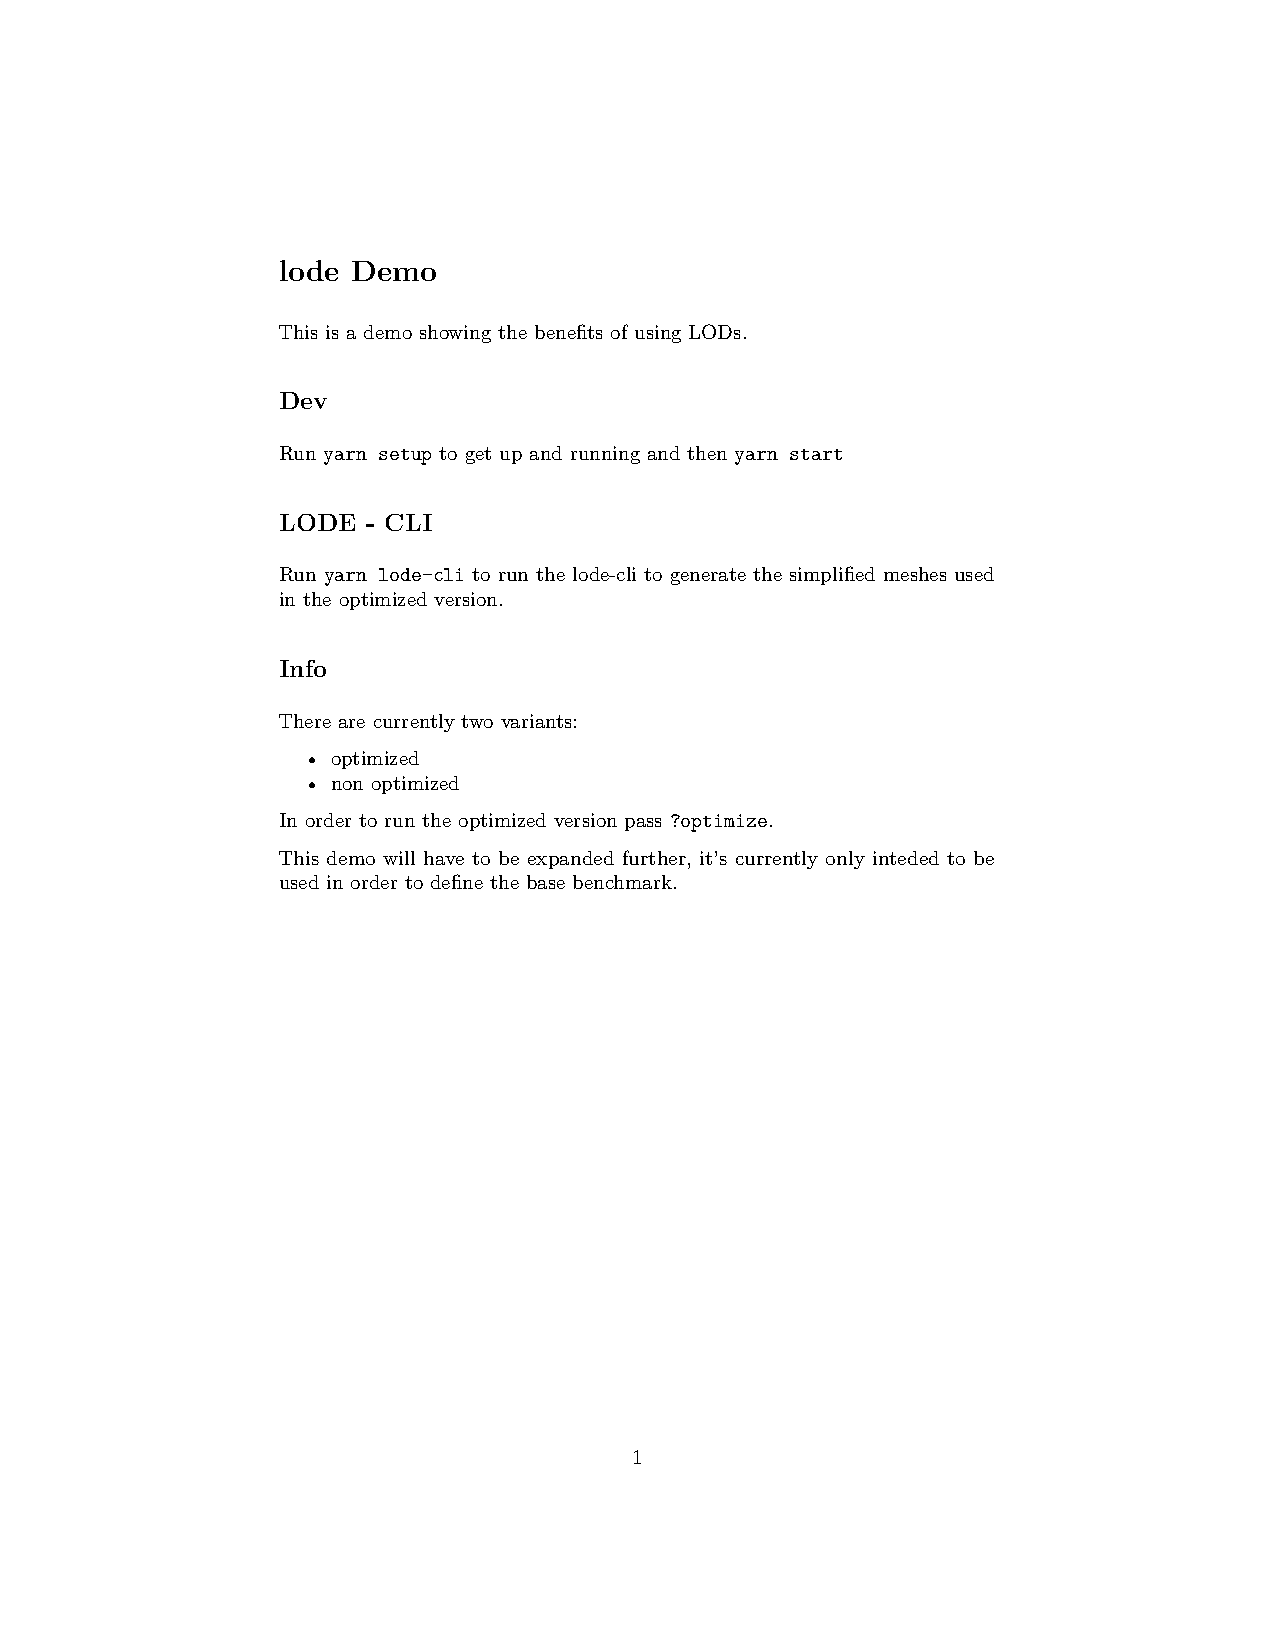
\includepdf[pagecommand={},scale=0.92,pages=-]{../ressources/packages/demo.pdf}
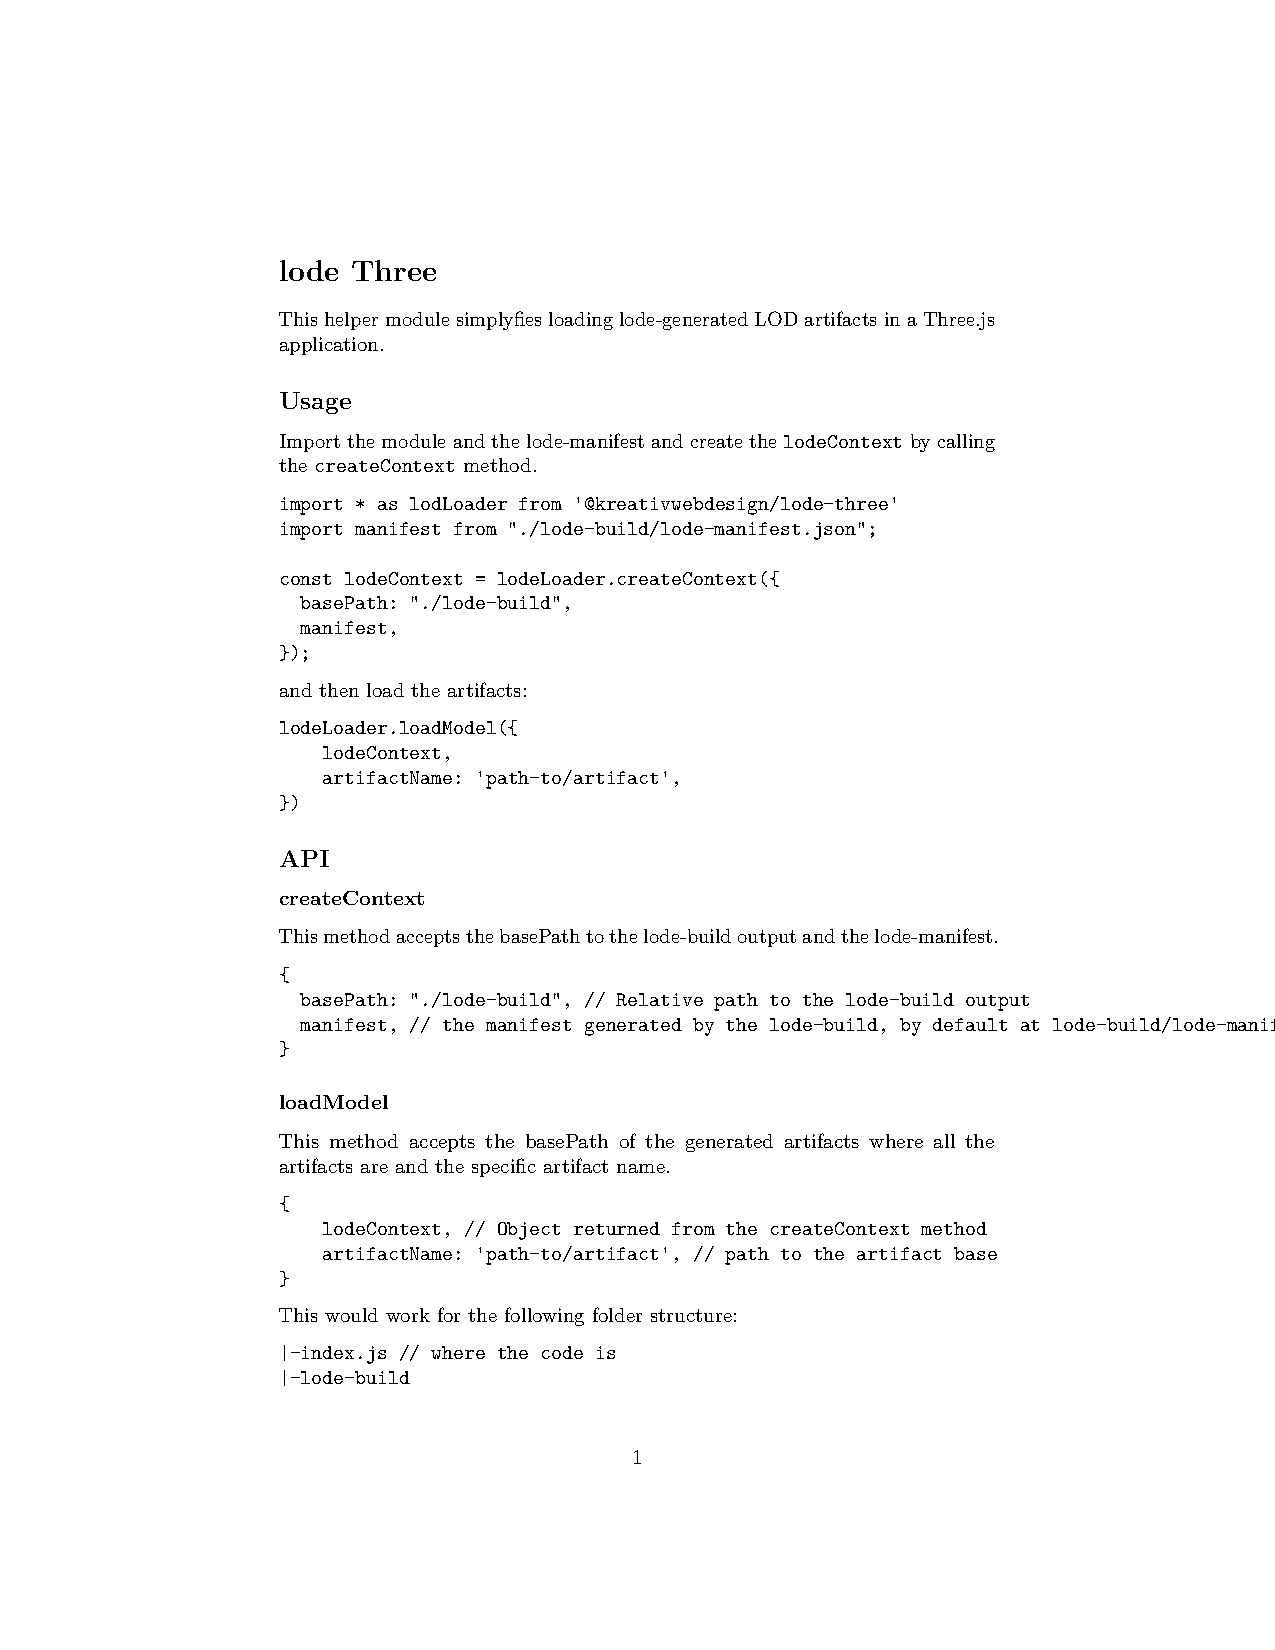
\includepdf[pagecommand={},scale=0.92,pages=-]{../ressources/packages/lode-three.pdf}
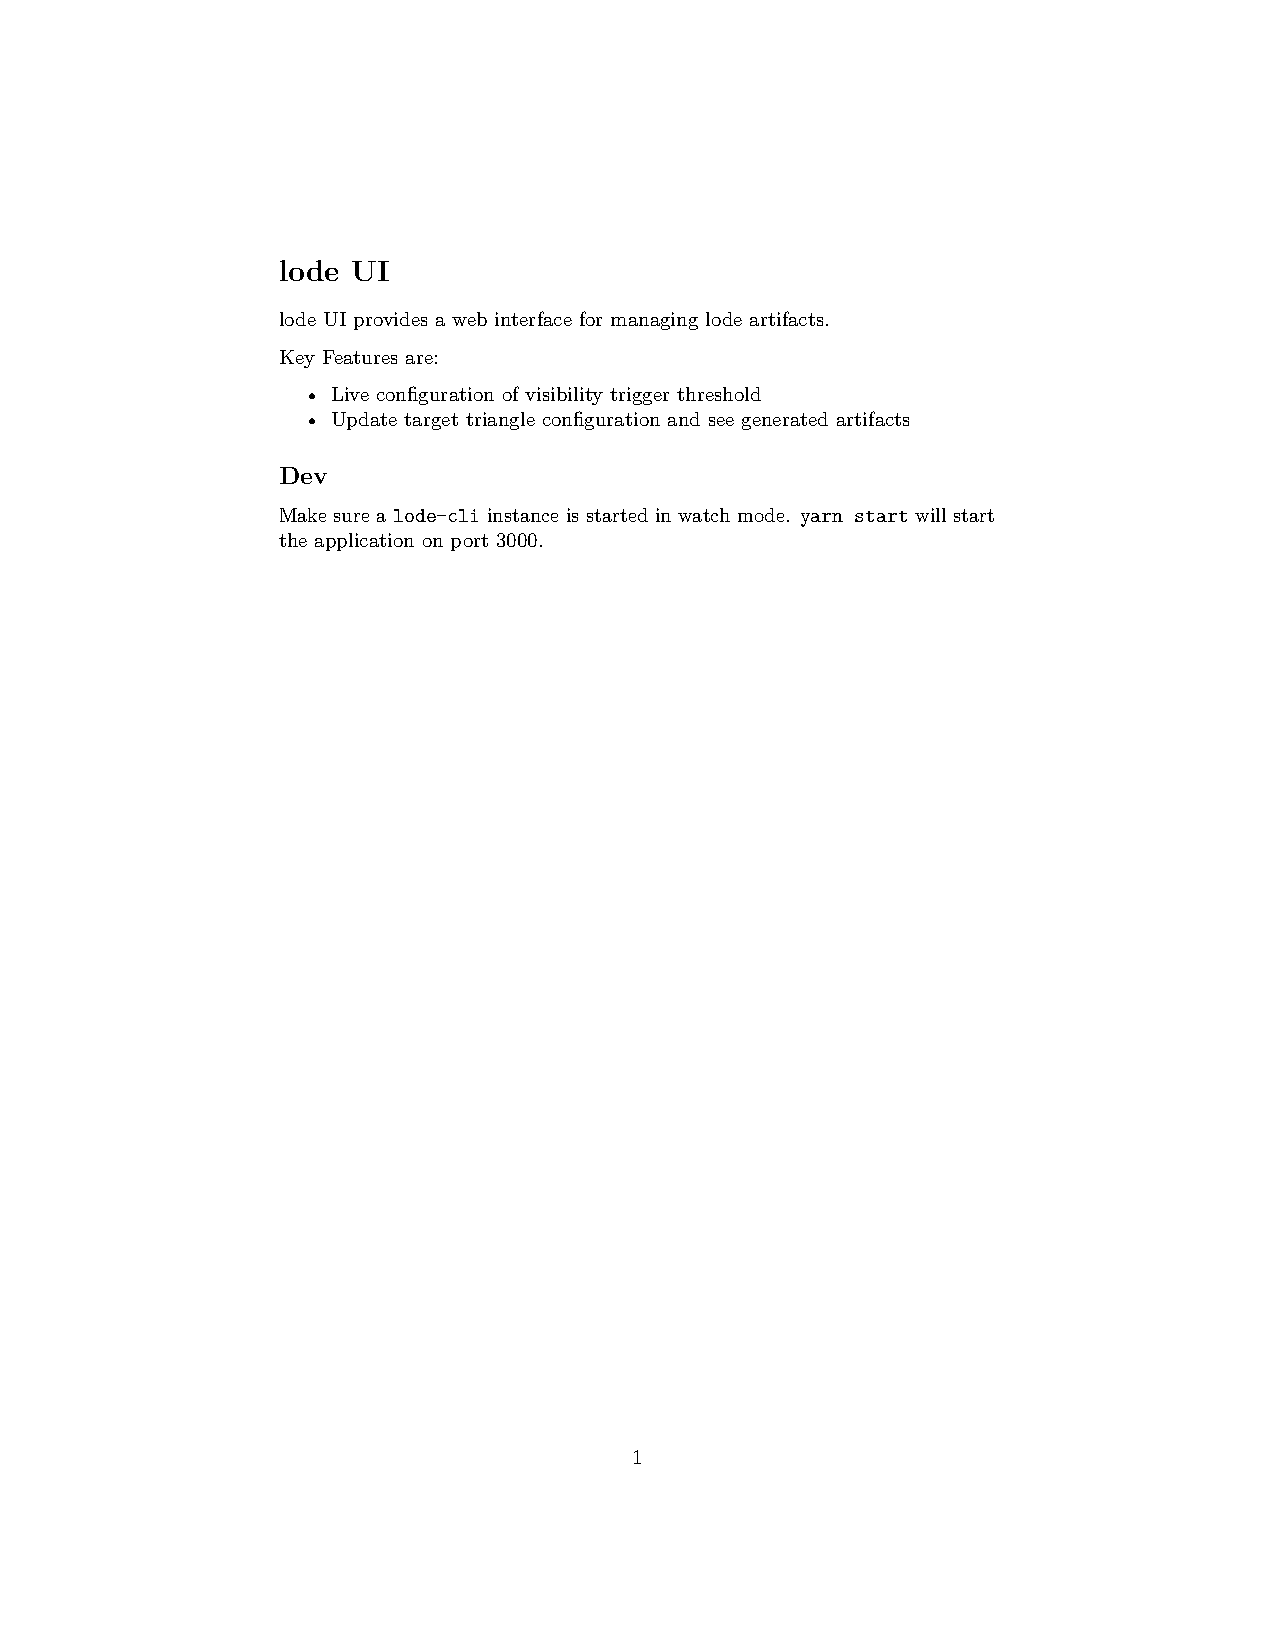
\includepdf[pagecommand={},scale=0.92,pages=-]{../ressources/packages/lode-ui.pdf}
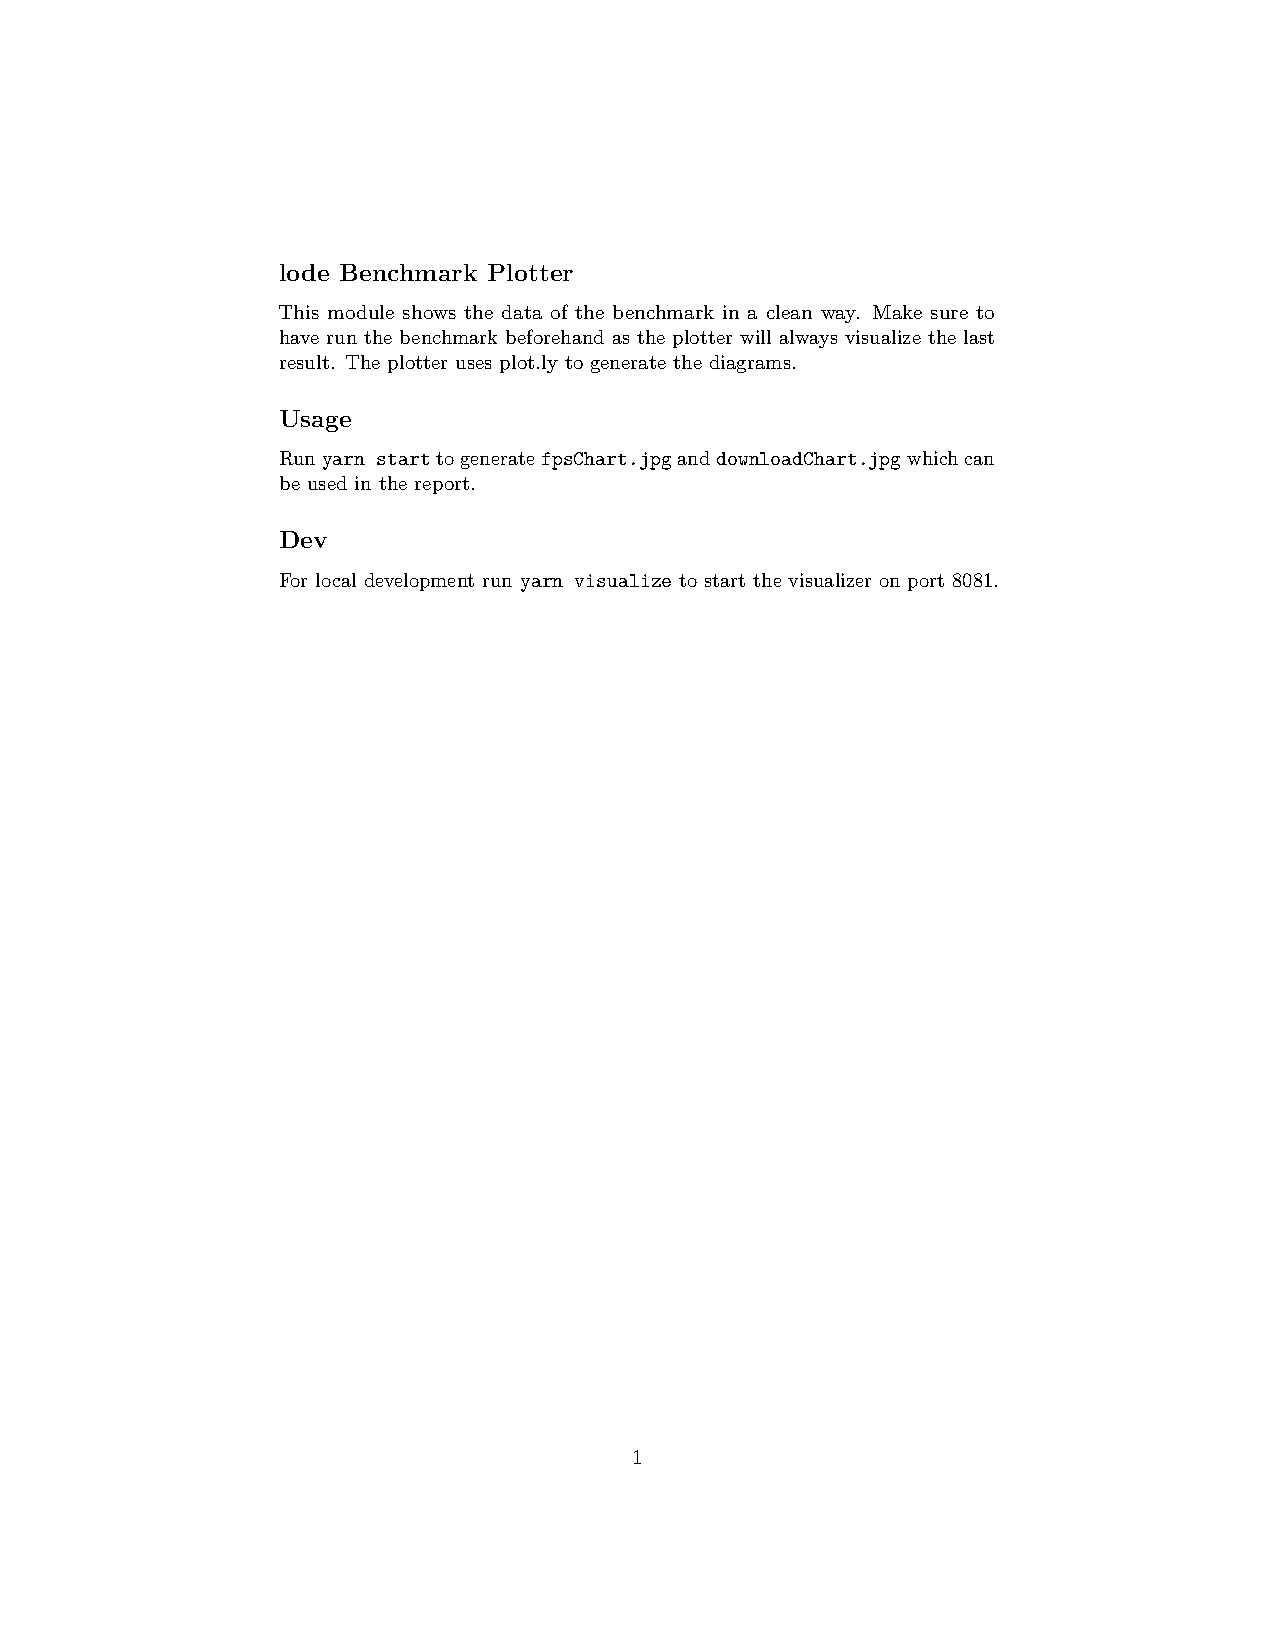
\includepdf[pagecommand={},scale=0.92,pages=-]{../ressources/packages/plotter.pdf}

\section{Benchmark Daten}
\begin{figure}[H]
  \begin{lstlisting}
    optimized fps: 59.9 (0.316 standard deviation)
    the value is with a confidence of 95% between 59.704 and 60.096
    baseline fps: 48.3 (0.483 standard deviation)
    the value is with a confidence of 95% between 48.001 and 48.599


    further information for interpreting data:

    gpuTotalTime:
    optimized: 108.406 (5.667 standard deviation)
    baseline: 336.718 (398.204 standard deviation)
    medianRenderLoopDuration:
    optimized: 2.067 (0.064 standard deviation)
    baseline: 1.394 (0.024 standard deviation)
    totalGpuEvents:
    optimized: 524.7 (26.081 standard deviation)
    baseline: 518.6 (17.89 standard deviation)
    totalModelLoadDuration:
    optimized: 1350.611 (42.677 standard deviation)
    baseline: 1233.288 (53.571 standard deviation)
    totalRenders:
    optimized: 300.4 (5.602 standard deviation)
    baseline: 232.3 (5.658 standard deviation)
  \end{lstlisting}
\caption{Durchlauf Benchmark auf MacBook Pro 2018}
\label{fig:benchmarkRun}
\end{figure}

\begin{figure}[H]
  \begin{lstlisting}
    CPU: 2.9 GHz Quad-Core Intel Core i7
    GPU: Radeon Pro 560 4 GB, Intel HD Graphics 630 1536 MB
    RAM: 16 GB 2133 MHz LPDDR3
  \end{lstlisting}
\caption{Hardwarespezifikation MacBook Pro 2018}
\label{fig:MarcbookProSpecification}
\end{figure}

\begin{figure}[H]
  \begin{lstlisting}
    optimized fps: 58.9 (0.316 standard deviation)
    the value is with a confidence of 95% between 58.704 and 59.096
    baseline fps: 11 (0.408 standard deviation)
    the value is with a confidence of 95% between 10.747 and 11.253


    further information for interpreting data:

    gpuTotalTime:
    optimized: 455.366 (139.317 standard deviation)
    baseline: 174.948 (111.763 standard deviation)
    medianRenderLoopDuration:
    optimized: 2.448 (0.537 standard deviation)
    baseline: 2.674 (0.603 standard deviation)
    totalGpuEvents:
    optimized: 490 (37.523 standard deviation)
    baseline: 150.5 (11.326 standard deviation)
    totalModelLoadDuration:
    optimized: 1201.504 (167.149 standard deviation)
    baseline: 1110.993 (140.091 standard deviation)
    totalRenders:
    optimized: 252.9 (56.432 standard deviation)
    baseline: 56.8 (5.245 standard deviation)
  \end{lstlisting}
\caption{Durchlauf Benchmark auf Dell mit Intel UHD Graphics 630}
\label{fig:windowsBenchmarkRun}
\end{figure}

\section{Projekt dokumentation}
\subsection{Zeitplan}
\begin{figure}[H]
  \centering
  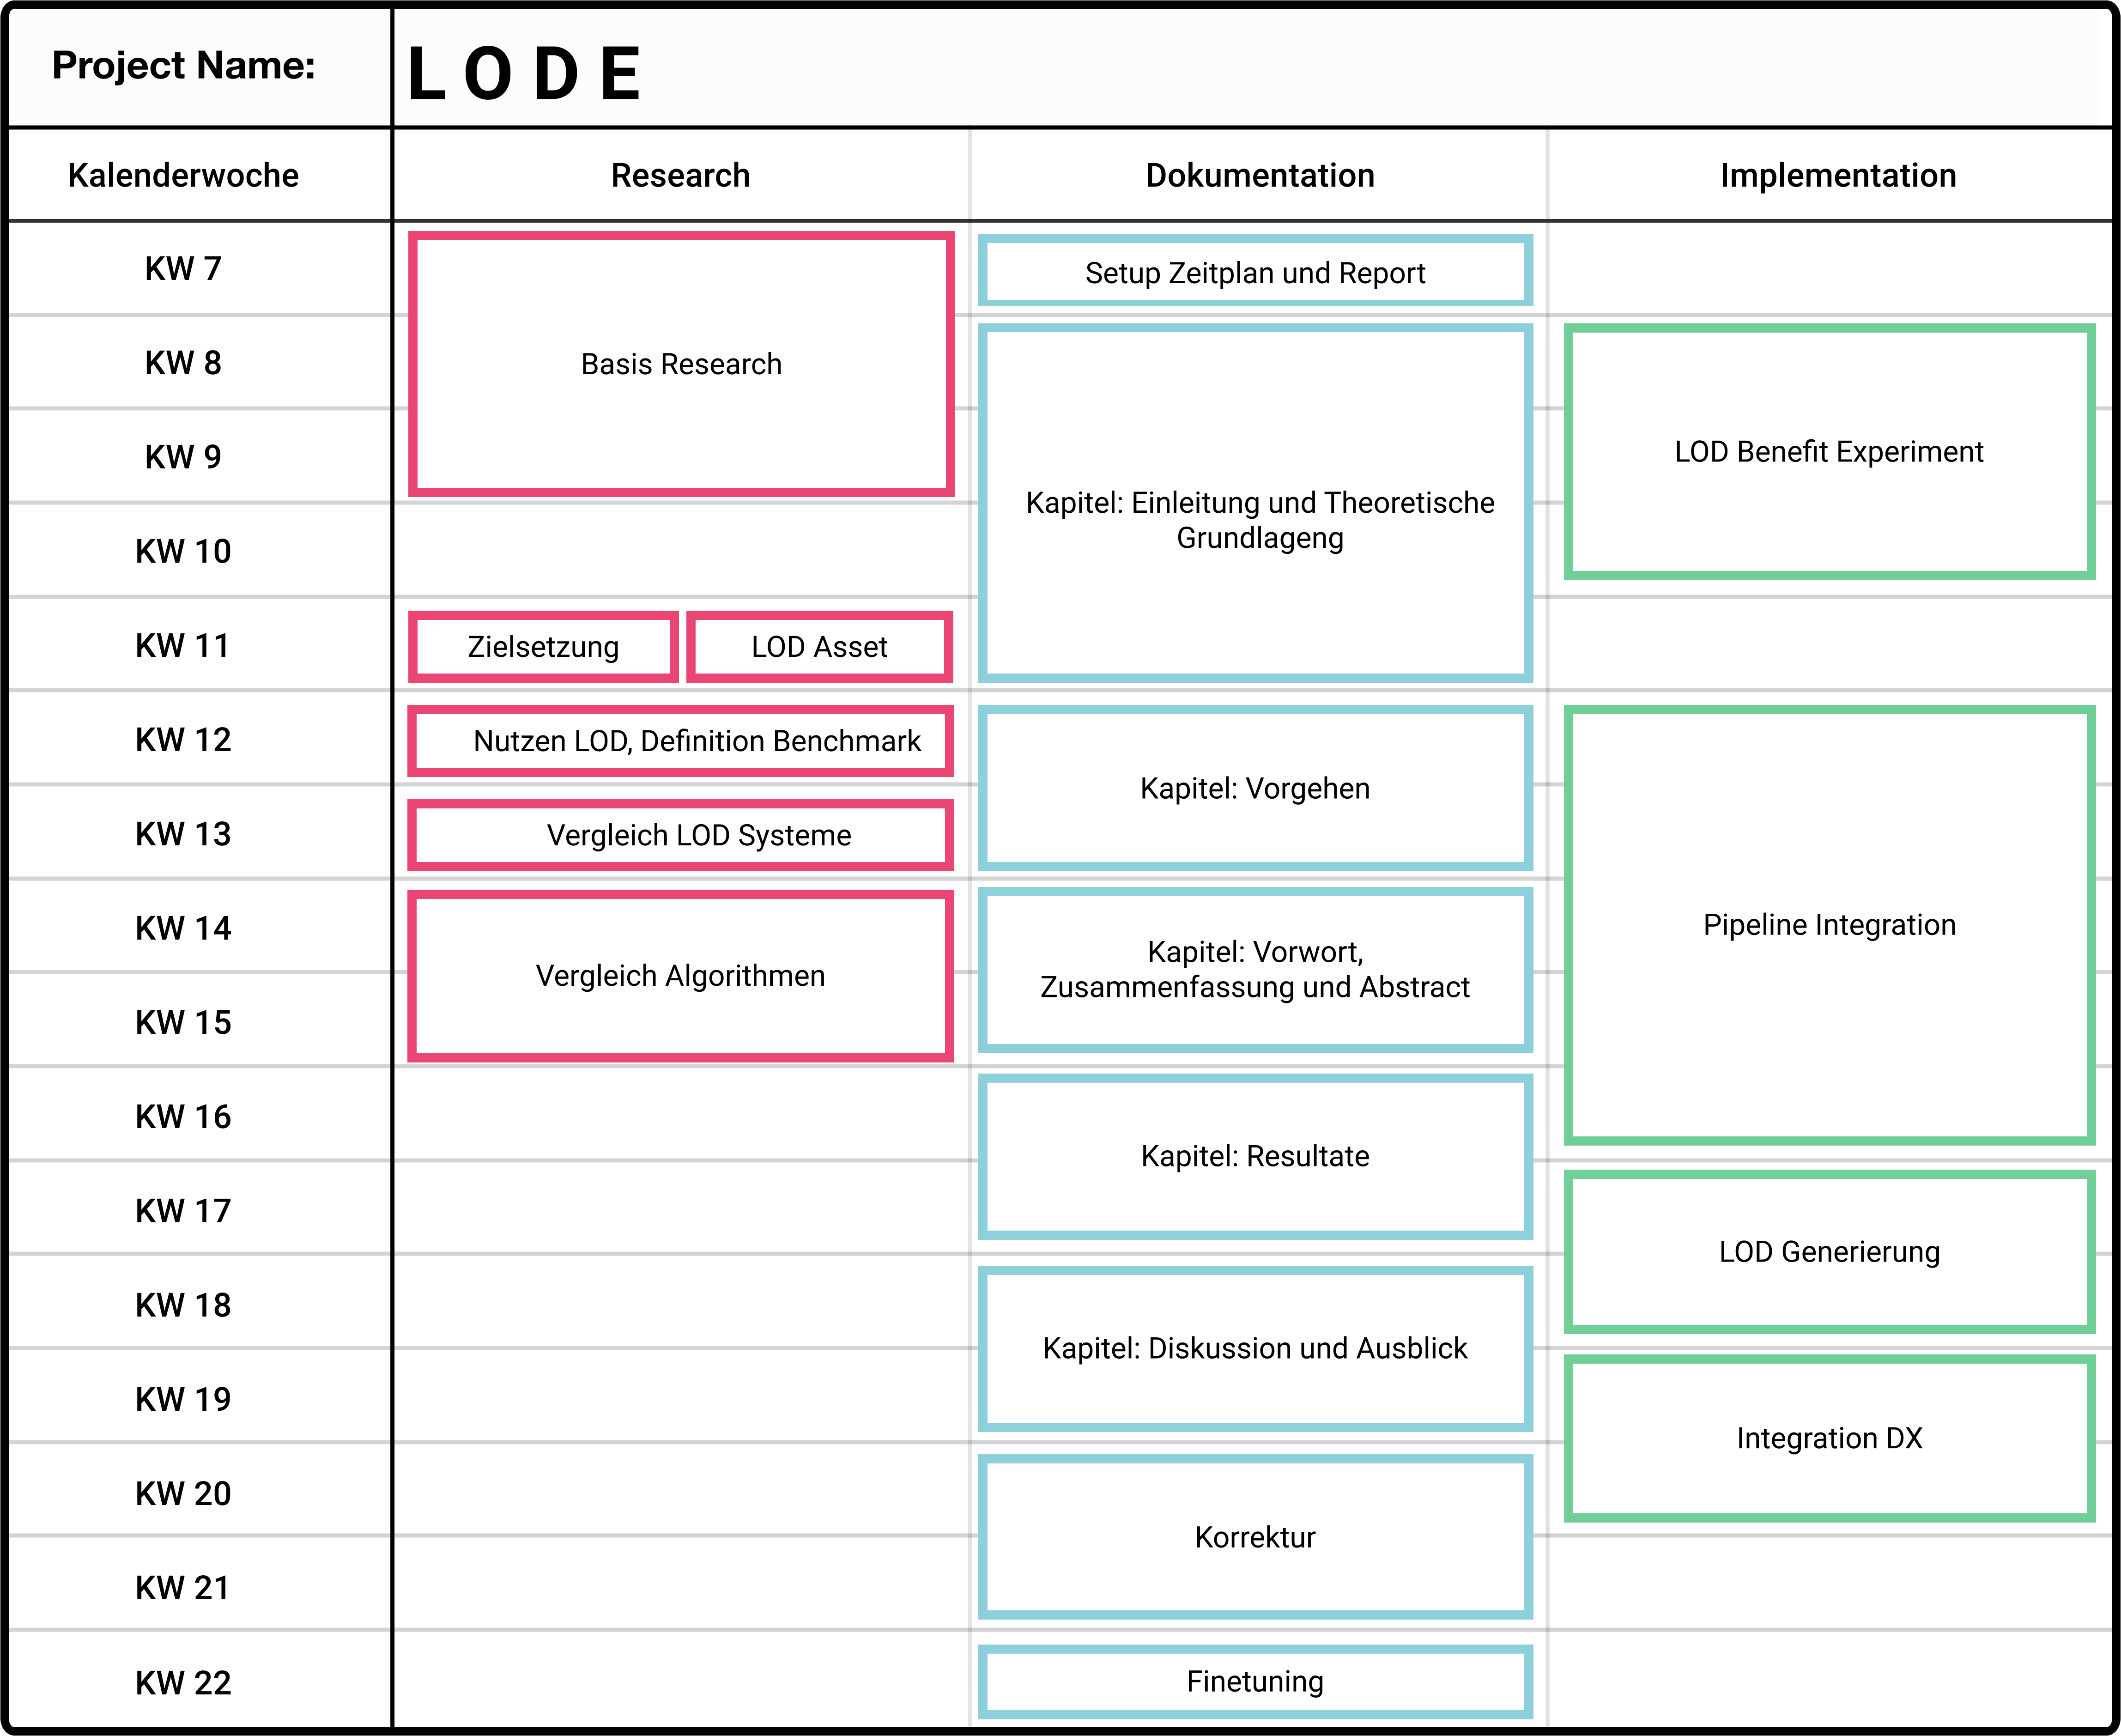
\includegraphics[width=1\columnwidth]{../ressources/zeitplan.png}
\end{figure}
\todo[inline]{@marc Besprechungsprotokolle}
